%!TEX root = ./main.tex

\chapter{Final results, discussion and conclusion} % (fold)
\label{sec:final_results_discussion_and_conclusion}

\section{Test environment} % (fold)
\label{sec:test_environment}

To test and investigate our results three test environments have been used, as shown in Table~\ref{sec:test_environment}.1. They all have different properties that are used to test different aspects of our algorithms. Test environment 3 has a normal Windows setup, with a graphics card that is used for both display rendering and CUDA computation. On the other hand, test environment 1, uses the same hardware, but is setup with a dedicated GPU\@. CUDA computations done on a environment without a dedicated GPU, is forced to split the resources with the running OS, which implies some restrictive properties. For instance, it is normal for an OS to kill long running GPU processes. On windows the normal timeout is around $30$ seconds. To get around this restriction some editing in regedit is necessary.

The last environment, number 2, is build on an Amazon web service (AWS) cloud instance. Using AWS, enables us to test implementations on a more powerful GPU, than what we currently have in our personal procession. The biggest advantage of the AWS GPU for our applications, is the increased on-board GPU memory. This enables us to store larger point clouds directly on the GPU. The increased number of CUDA cores, also makes it possible to test performance ratios, and different variants of resource distributions.

\begin{table}[ht]
\centering
    \begin{tabular}{|l|l|l|l|}
        \hline
        \textbf{Test envoronment} & \textbf{1}         & \textbf{2}       & \textbf{3}\\ \hline
        \textbf{OS}               & Ubuntu 14.04       & Ubuntu 12.04     & Windows 7  \\ \hline
        \textbf{OS type}          & x64                & x64              & x64     \\ \hline
        \textbf{Kernel}           & 3.13.0-24-generic  & 3.2.0-58-virtual & Windows 7      \\ \hline
        \textbf{CPU}              & i7-2600K           & E5-2670          & i7-2600K       \\ \hline
        \textbf{CPU memory}       & 7.8 Gb             & 16 Gb            & 7.8 Gb \\ \hline
        \textbf{GPU}              & GeForce GTX 560 Ti & NVIDIA GRID K520 & GeForce GTX 560 Ti      \\ \hline
        \textbf{GPU memory}       & 1024 Mb            & 4095 MB          & 1024 Mb      \\ \hline
        \textbf{Dedicated GPU}    & Yes                & Yes              & No       \\ \hline
        \textbf{CUDA cores}       & 384                & 1536             & 384       \\ \hline
        \textbf{CUDA capability}  & 2.1                & 3.0              & 2.1       \\ \hline
        \textbf{CUDA driver}      & 5.5                & 5.5              & 5.5       \\ \hline
        \textbf{CUDA runtime}     & 5.5                & 5.5              & 5.5       \\ \hline
    \end{tabular}
    \caption{Tabulated information about the three test environments.}
    \label{tbl:test_envoronments}
\end{table}

All tests was run multiple times and averaged, to get more accurate results. It should also be noted that it is common practice to warm up the GPU before any test, because it may take as long time for the CUDA runtime to create a CUDA context, as launching the kernel itself.

All tests used synthetic data, generated as uniformly distributed random points in a unit cube. Where needed, random points was generated and stored to disk. This data could then be used as the source for several different tests, eliminating deviation in tests used for comparison of between different implementations.

Using uniformly distributed data is not necessarily a good representation for all real world point cloud data, but this should not affect our results for the brute-force and k-d tree build algorithm, given that these algorithms have a non-stochastic runtime, not affected by the location of our test points. Given that we always balance the k-d tree, the k-d query algorithm should not be significantly affected by changing the point distribution, although slight deviations might be observed.

Due to the reasons above, and the available time for this thesis, we have chosen not to include other point distributions in our tests, but this could be an interesting study for further work.
% section test_envorinment (end)

\section{Final results and discussion} % (fold)
\label{sec:final_results_and_discusstion}

During the development of our algorithms, we have presented many intermediate results, in order to argument for the design and implementation choices made. In this section, we will present our final results for the GPU parallelized brute force, GPU parallelized and CPU parallelized k-d tree based kNN algorithm.

The different research questions stated during development of our algorithms are revisited, and answered are given, based on the presented results.

\subsection{Solving the kNN problem} % (fold)
\label{sub:solving_the_knn_problem}

In Section~\ref{sub:investigation_of_a_brute_force_approach_based_on_garcia} we started on our quest for a faster kNN search, by investigating a possible brute-force algorithm, pioneered by Garcia et.al. The following research question was asked. 

\textbf{RQ~\ref{rq:brute_force_performance}.} \emph{Can high performance be achieved by a parallel brute force kNN algorithm on large point clouds.}

In order to discuss this question, we have to clarify what we consider to be high performance in this context. The work of Garcia et.al\@. contains the fastest brute force algorithm, for solving the kNN problem, we have found in current literature. We would therefore consider a kNN algorithm to have high performance, if it is able to solve the kNN problem for point cloud data, in the 3D format specified by TSI, at comparable speeds to the algorithm developed by Garcia et.al. 

Although the algorithm developed by Garcia et.al\@. is the fastest brute force algorithm we have managed to find, this is not as a high benchmark as it might initially seem. The algorithm developed by Garcia et.al\@. is optimized for solving the kNN problem for a more general version of the kNN problem than required by TSI\@. Where we are only concerned with solving the kNN problem for three dimensions, Garcia's algorithm will solve problems stated in any dimension. Given that we solve a more restricted version of the kNN problem, any less than comparable speeds to the implementation made by Garcia et.al\@. could not be considered to be of high performance in our eyes.

\begin{figure}[ht!]
    \centering
    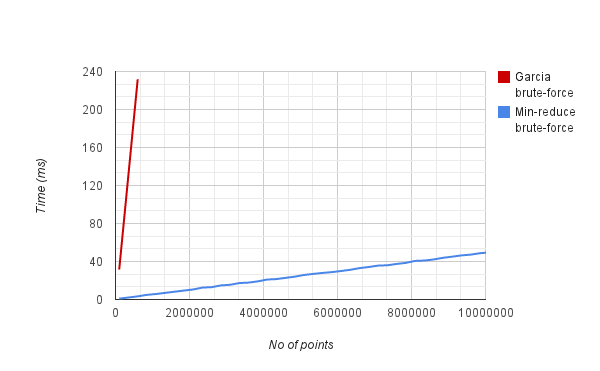
\includegraphics[width=120mm]{../gfx/fin-garcia-vs-min-reduce.png}
    \caption{Comparison of brute-force algorithm developed by Garcia et.al\@. and min-reduce based brute-force algorithm developed in this thesis. $k$ is fixed at 10 and $m$ is increasing.}
    \label{fig:fin-garcia-vs-min-reduce}
\end{figure}

In Section~\ref{sub:continuing_on_garcia_s_path}, we discussed Figure~\ref{fig:brute_force}. As a reminder, part of this figure is presented as Figure~\ref{fig:fin-garcia-vs-min-reduce}, which shows the result of a comparison between the brute force algorithm developed by Garcia et.al\@. and our min-reduce brute-force algorithm developed in Section~\ref{sub:continuing_on_garcia_s_path}. The test is performed with a low value for $k=10$, and focuses on performance for large values of number of points, $m$. In this test, our min-reduce brute-algorithm is shown to be almost $70$ times faster than the algorithm developed by Garcia et.al\@. In addition, it is capable of solving the kNN problem for much larger values of $m$.

We therefore conclude that RQ~\ref{rq:brute_force_performance} can be answered with yes. High performance can be achieved with a brute-force based algorithm.

In Section~\ref{sub:application_of_kd_trees_to_the_knn_problem} we introduced the k-d tree, a data-structure with a known \BigO{log(m)} nearest neighbor query algorithm. We therefore presented a new research question, which we try to answer in Figure~\ref{fig:final-knn-kd-vs-bf}.

\textbf{RQ~\ref{rq:serial-kd-tree}.} \emph{It is possible to use a k-d tree to increase the performance of kNN queries, compared to a parallel brute force solution?}

\begin{figure}[ht!]
    \centering
    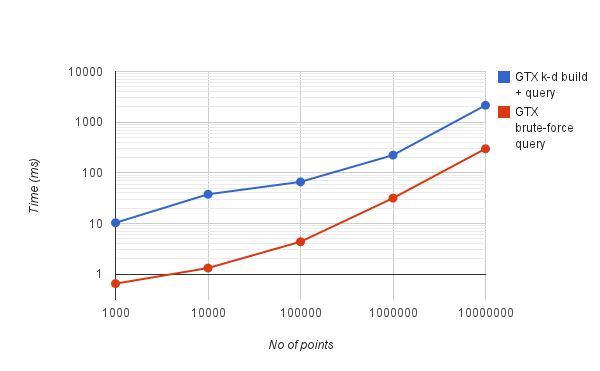
\includegraphics[width=120mm]{../gfx/final-knn-kd-vs-bf.png}
    \caption{Comparison of min-reduce brute-force and k-d tree based algorithms for solving the kNN problem for $k=100$ and increasing $m\le1e7$.}
    \label{fig:final-knn-kd-vs-bf}
\end{figure}

The graph compares the runtime of the k-d tree build and query algorithms developed in Section~\ref{sec:the_quest_for_a_faster_knn_search}, with the min-reduce brute-force algorithm. All test data is generated using test environment 1.

Figure~\ref{fig:final-var-knn-kd-vs-bf} compares the same two algorithms, but for a fixed value of $m$, and increasing value of $k$. This test is also performed using test environment 1.

\begin{figure}[ht!]
    \centering
    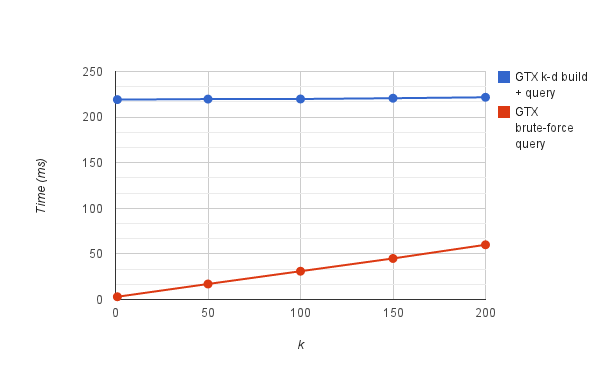
\includegraphics[width=120mm]{../gfx/final-var-knn-kd-vs-bf.png}
    \caption{Comparison of min-reduce brute-force and k-d tree based algorithms for solving the kNN problem for $m=\numprint{1.0e6}$ and increasing $k\le200$.}
    \label{fig:final-var-knn-kd-vs-bf}
\end{figure}

Both Figure~\ref{fig:final-knn-kd-vs-bf} and \ref{fig:final-var-knn-kd-vs-bf} shows that this algorithm is slower than a brute force approach. This answers RQ~\ref{rq:serial-kd-tree}. In order to solve the kNN problem, the k-d tree based solution first has to construct the k-d tree, then query for the closest points. Given that our previous calculation shows that the time complexity of the k-d tree build algorithm is larger than the time-complexity for the brute-force algorithm, this result should come as no surprise. Constructing the k-d data-structure for a single query is simply a waste of resources, if just one kNN query is to be performed.
% subsection solving_the_knn_problem (end)

\subsection{Solving the All-kNN problem} % (fold)
\label{sub:solving_the_all_knn_problem}

The All-kNN problem was studied in both relation to the brute-force algorithm and the k-d tree based algorithm. In Section~\ref{sub:continuing_on_garcia_s_path} we proposed RQ~\ref{rq:brute_force_Q-kNN}. We also wanted to compare our parallel k-d tree based algorithm to the brute-force algorithm, postulated in RQ~\ref{rq:serial-kd-tree-all-knn}.

\textbf{RQ~\ref{rq:brute_force_Q-kNN}.} \emph{Can a parallel brute force kNN algorithm be fast enough to solve the All-kNN problem within reasonable time?}

\textbf{RQ~\ref{rq:serial-kd-tree-all-knn}.} \emph{It is possible to use a k-d tree to increase the performance of All-kNN queries, compared to a parallel brute force solution?}

Figure~\ref{fig:final-all-knn-gpu-vs-cpu-vs-bf} compares the runtime of the min-reduce brute-force algorithm to the k-d tree based algorithm, for increasing values of $m\le1e7$, and a fixed value of $k=100$. The data series for the min-reduce algorithm is estimated from the data obtained in Figure~\ref{fig:final-knn-kd-vs-bf}. This estimation is valid, since all GPU resources are used to perform one kNN query, when using the brute-force algorithm. Solving the All-kNN problem with the brute-force algorithm, can therefore only be performed as repeated application of the brute-force kNN algorithm, given a reasonable hardware setup, with one CUDA enabled GPU\@.

The data series for the k-d tree based algorithms are, on the other hand, generated from actual runtime results. This is due to the k-d query algorithm being developed as a parallelized Q-kNN query, where individual kNN queries are parallelized, instead of one single kNN query, as is the case with the brute-force algorithm. We have developed two different implementations of this k-d tree based Q-kNN query. One parallelized on the GPU, annotated with GTX k-d build + m queries, and one parallelized on the CPU, annotated with CPU k-d build + m queries. All tests was performed using test environment 1.

\begin{figure}[ht!]
    \centering
    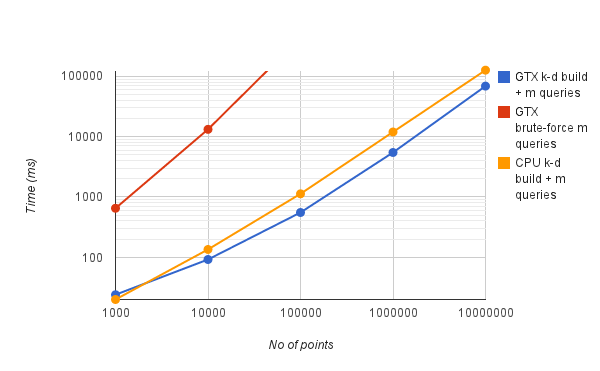
\includegraphics[width=120mm]{../gfx/final-all-knn-gpu-vs-cpu-vs-bf.png}
    \caption{Comparison of min-reduce brute-force and k-d tree based algorithms with CPU and GPU parallelized query. The graph compares runtime for solving the All-kNN problem for $k=100$ and increasing $m$.}
    \label{fig:final-all-knn-gpu-vs-cpu-vs-bf}
\end{figure}

Figure~\ref{fig:final-var-all-knn-kd-vs-bf} compares the GPU parallelized k-d tree algorithm, with the parallel brute force algorithm, for a fixed value of $m$, and increasing values for $k\le200$. Test environment 1 is also used in this comparison.

\begin{figure}[ht!]
    \centering
    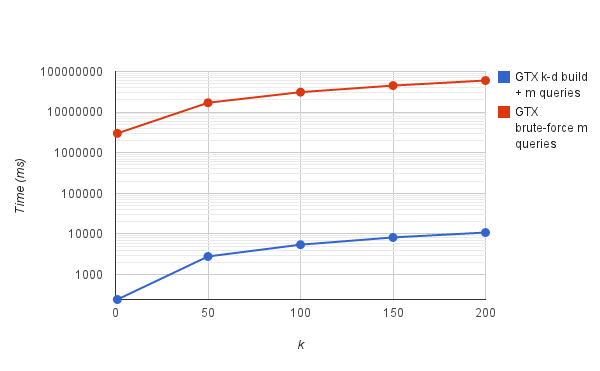
\includegraphics[width=120mm]{../gfx/final-var-all-knn-kd-vs-bf.png}
    \caption{Comparison of min-reduce brute-force and GPU parallelized k-d tree based algorithms for solving the All-kNN problem for $m=1e6$ and increasing $k\le200$.}
    \label{fig:final-var-all-knn-kd-vs-bf}
\end{figure}

Both graphs clearly shows the benefit of using a k-d tree based algorithm for solving the All-kNN problem. As discussed in Section~\ref{sub:testing_a_serial_k_d_tree_based_knn_solver}, part of this increased performance over a brute-force based solver, is due to the k-d query algorithm being able to execute in \BigO{log(m)} time. Since we do not have to rebuild the tree between the individual kNN queries when performing a All-kNN query, the reduction in query runtime has larger impact on the overall execution of the algorithm.

Another important factor is that each k-d kNN query, is parallelized. This can be done for a k-d based query algorithm, since the resource requirements for each individual kNN query is lower than for the brute-force algorithm. These two improvements combined, result in an algorithm that is capable of solving the All-kNN problem for values of $m$ and $k$, that would not be feasible with a brute-force algorithm. This answers RQ~\ref{rq:serial-kd-tree-all-knn}.

Figure~\ref{fig:final-all-knn-gpu-vs-cpu-vs-bf} shows that the brute-force algorithm is capable of solving the All-kNN for small point clouds, although significantly slower than the k-d tree based algorithm. With a point cloud containing just $10000$, the brute force algorithm will take at least $10$ s to execute, compared to the $100$ ms required by the k-d tree based algorithm. Although slow, for low values of $m$, the brute-force algorithm computes the answer within arguably reasonable time. When $m$ is increased, this changes. For a point cloud of size $1e7$, the brute-force algorithm would require about $3e9$ ms to compute the answer, or almost 34 days. This would most certainly not be considered to be within reasonable time. The answer to RQ~\ref{rq:brute_force_Q-kNN} is therefore dependent on the size of $m$. It can be argued that the brute-force algorithm is capable, but not the best alternative, for solving the All-kNN problem for small values of $m$.

In Figure~\ref{fig:final-all-knn-gpu-vs-cpu-vs-bf} the impression is that the GPU and CPU parallelized k-d algorithms performs similarly. We will therefore investigate additional results, to get a better understanding of how they compare.

Figure~\ref{fig:v17-gpu-vs-cpu} compares the difference between the CPU and the GPU parallelized k-d query algorithm. Test environment 1 is again used.

\begin{figure}[ht!]
    \centering
    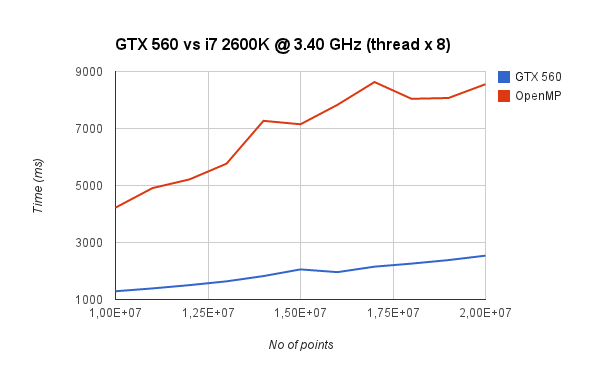
\includegraphics[width=120mm]{../gfx/v17-gpu-vs-cpu.png}
    \caption{Comparison of runtime for GPU (GTX 560) and CPU (OpenMP) parallelized k-d tree based n query.}
    \label{fig:v17-gpu-vs-cpu}
\end{figure}

In Figure~\ref{fig:v17-gpu-vs-cpu} the CPU based parallelization is slower than the GPU based parallelization. Although smaller than the difference between the brute-force algorithm and the k-d tree based algorithm, it is still a significant difference. This indicates, that for this algorithm, the benefit of having faster individual cores, and less overhead related to memory transfer on the CPU, is not enough to offset the drawback of the CPU has a lot fewer parallel cores than the GPU\@. Using the GPU parallelized version, where possible, is therefore recommended.
% Maybe a final graph with All-kNN, k = 100 for very large values of m? Just some data points?
% subsection solving_the_all_knn_problem (end)

\subsection{Parallelization performance increase} % (fold)
\label{sub:parallelization_performance_increase}
 Continuing on our quest for a fast kNN search, a parallelization of the k-d tree build was introduced with RQ~\ref{rq:parallel_build}, in Section~\ref{sec:development_of_a_parallel_k_d_tree_build_algorithm}.

\textbf{RQ~\ref{rq:parallel_build}.} \emph{It is possible to parallelize the k-d tree build algorithm, in such a way that it gives a significant speed improvement compared to the serial algorithm.}

The resource question is based around the complex nature of the k-d tree build, and the uncertainty of a acceptable parallel speedup. This question was investigated though implementation prototypes, together with a thorough discussion about the parallelization strategy and the intermediate results. 

\begin{figure}[ht!]
    \centering
    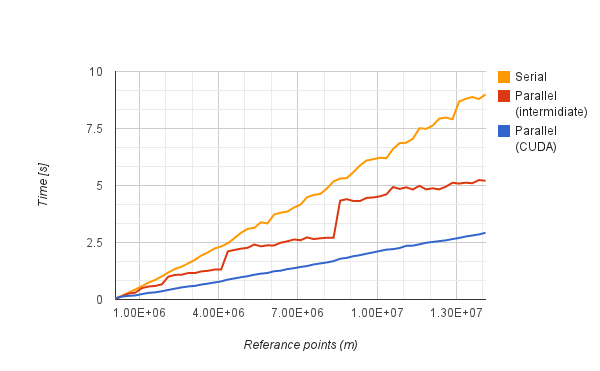
\includegraphics[width=120mm]{../gfx/final_tree_build.png}
    \caption{Comparison between serial and parallel k-d tree build performance.}
    \label{fig:final_tree_build}
\end{figure}

Figure~\ref{fig:final_tree_build} tries to answer RQ~\ref{rq:parallel_build}, by comparing the serial and parallel k-d tree build implementation. Both graphs follows the same trend, which correlates with the shared time complexity of \BigO{m\ log(m)}. We see that the impact of the parallel overhead is decreasing as the problem size increase, and the profit of multiple cores is getting more and more be dominant. Resulting in a faster parallel implementation.

To get a better picture of the parallel improvement, it is natural to talk about parallel speedup. Figure~\ref{fig:final_tree_build_speedup} shows how the parallel speedup develops, as the problem size increase. Here we see that the speedup starts below $1$, indicating that the serial version is faster then the parallel version, but from Figure~\ref{fig:final_tree_build} one can see that the time to build such small k-d trees is almost negligible. As the problem size increase, the trend quickly changes, until the speedup flattens out. The speedup increases as the problem size allows utilization of more and more threads, until the limit is reached, and the curve flattens out into a lower gradient.      

\begin{figure}[ht!]
    \centering
    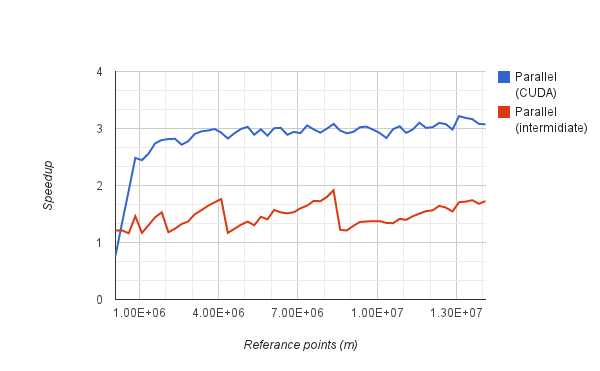
\includegraphics[width=120mm]{../gfx/final_tree_build_speedup.png}
    \caption{Parallel speedup for the k-d tree implementation for varying values of $m$.}
    \label{fig:final_tree_build_speedup}
\end{figure}

With the complex nature if a k-d tree build process, a speedup of three is acceptable, and we categorize it as a significant improvement, which answer RQ~\ref{rq:parallel_build}. 


RQ~\ref{rq:parallel_query} proposed the next topic of our quest, namely the parallelization of the All-kNN query. 

\textbf{RQ~\ref{rq:parallel_query}.} \emph{It is possible to parallelize the All-kNN query algorithm, in such a way that it gives a significant speed improvement compared to the serial algorithm.}

\begin{figure}[ht!]
    \centering
    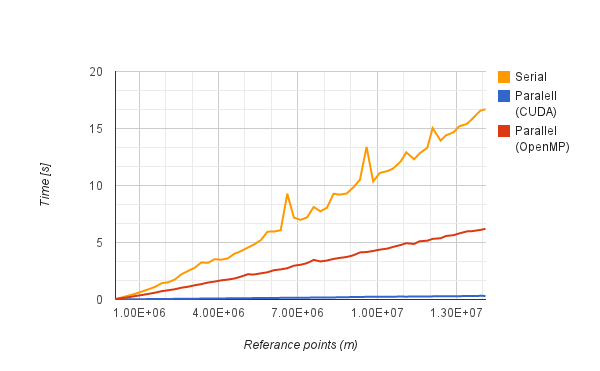
\includegraphics[width=120mm]{../gfx/final_kd_search.png}
    \caption{Comparison between serial and parallel All-kNN query performance.}
    \label{fig:final_kd_search}
\end{figure}

Figure~\ref{fig:final_kd_search} visualize the results from the two different parallel All-kNN query implementations, CUDA and OpenMP, compared to the serial version. The linear trend, also found in the k-d tree build algorithm, is not surprising, as the time complexity for all algorithms are \BigO{m\ log(m)}. The parallel improvement is only shown in the gradient these slopes have, which is reasonable, because the work is only divided amongst more cores. In both OpenMp and CUDA the parallel improvement is significant.

\begin{figure}[ht!]
    \centering
    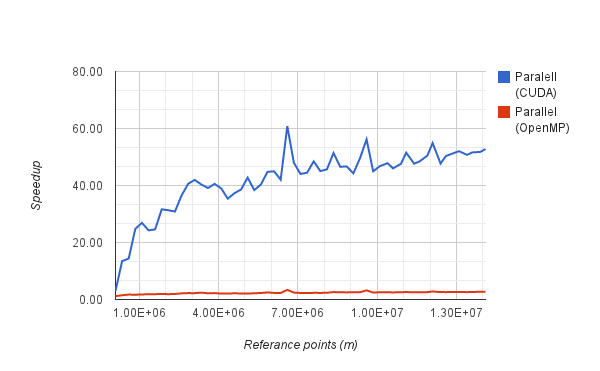
\includegraphics[width=120mm]{../gfx/final_kd_search_speedup.png}
    \caption{Parallel speedup comparison for the All-kNN query between the CUDA and OpenMP implementation.}
    \label{fig:final_kd_search_speedup}
\end{figure}

If we look at the parallel speedup, shown in Figure~\ref{fig:final_kd_search_speedup}, we can again conclude that the OpenMP version is outperformed by the CUDA implementation. The trend resembles what we saw in the k-d tree build parallelization, only this time the speedup goes towards $50$ in the CUDA version. This correlations perfectly with the discussion, in Section~\ref{sub:parallelization_strategy}, about the parallelization strategy and how easily the work could be partitioned.      

An interesting note is that this speedup is lower then in both our and Garcia's\cite{Garcia2008} brute force implementations, which implies that speedup don't equal a fast implementations. It only implies a good parallel performance increase, compared to the serial algorithmic in use.

This answers RQ~\ref{rq:serial-kd-tree}, and we conclude that our All-kNN query has a significant parallel improvement.
% subsubsection parallelization_of_the_k_d_tree_build (end)

% subsection parallelization_performance_increase (end)
% section final_results_and_discusstion (end)

\clearpage

\section{Conclusion} % (fold)
\label{sec:conclusion}

In this thesis, we have investigated the possible benefits of using general-purpose computing on graphics processing units, in order to speed up the execution of calculations in engineering applications. We have investigated this topic, by improving the performance of point cloud analysis in engineering software developed by TechnoSoft Inc.

By utilizing the parallelization possibilities offered by CUDA enabled GPUs, and optimizing our algorithms for 3D point cloud data, we have been able to develop fast algorithms for solving the kNN and All-kNN problem.

The parallel brute-force algorithm developed in this thesis, is $70$ times faster than the brute-force algorithm developed by Garcia et-al. \cite{Garcia2008} on comparable problem sizes. Considering the algorithm developed by Garcia et.al. is significantly faster than conventional libraries, being up to $407$ times faster than Matlab, and up to $148$ times faster than ANN \citep[Table 1]{Garcia2008}, this is a notable result.

A parallel k-d tree based Q-kNN algorithm has also been developed in this thesis, and optimized for solving the All-kNN problem. The parallel k-d tree based algorithm is able to solve the All-kNN problem $300$ times faster than the parallel brute force implementation, and this could enable All-kNN analysis of much larger point clouds than was previously feasible.

In addition, all algorithms has been implemented with memory scalability in mind, resulting in a finished library of algorithms, which solves kNN and All-kNN problems faster, and for larger point clouds, than other alternatives, known from literature. This library is currently being integrated into point cloud analysis software at TechnoSoft Inc.

In conclusion, our results indicate that large runtime improvements can be achieved in engineering software, by utilizing the parallel performance of GPUs to speed up time-consuming algorithms.
% section conclusion (end)
